\documentclass{beamer}
\usepackage{graphics,color}
\usepackage{textcomp}
\usepackage{xcolor}
\usepackage{pgfplots}
\usepackage{pgfplotstable}
\usepackage{booktabs}
\usepackage{array}
\usepackage{colortbl}
\usepackage{amsmath,mathpazo}
\usepackage[utf8]{inputenc}
\usepackage{multicol}

\newcommand\blfootnote[1]{%
  \begingroup
  \renewcommand\thefootnote{}\footnote{#1}%
  \addtocounter{footnote}{-1}%
  \endgroup
}



\title{Buck Converter Power Train in Skywater 130nm}
\author{Teo Ene \\
  Ross Thompson}
\institute{Oklahoma State University}
\date{April 2022}

\usetheme{osu}

\begin{document}

\frame{\titlepage}

\begin{frame}
  \frametitle{Overview}
  \begin{itemize}
  \item Topology
  \item Design Parameters
  \item Circuit
  \item Deadtime
  \item Specification
  \end{itemize}
\end{frame}

\begin{frame}
  \frametitle{Topology and Design Goals}
\end{frame}

\begin{frame}
  \frametitle{Passive Components}
\end{frame}

\begin{frame}
  \frametitle{Frequency}
\end{frame}

\begin{frame}
  \frametitle{Buck}
  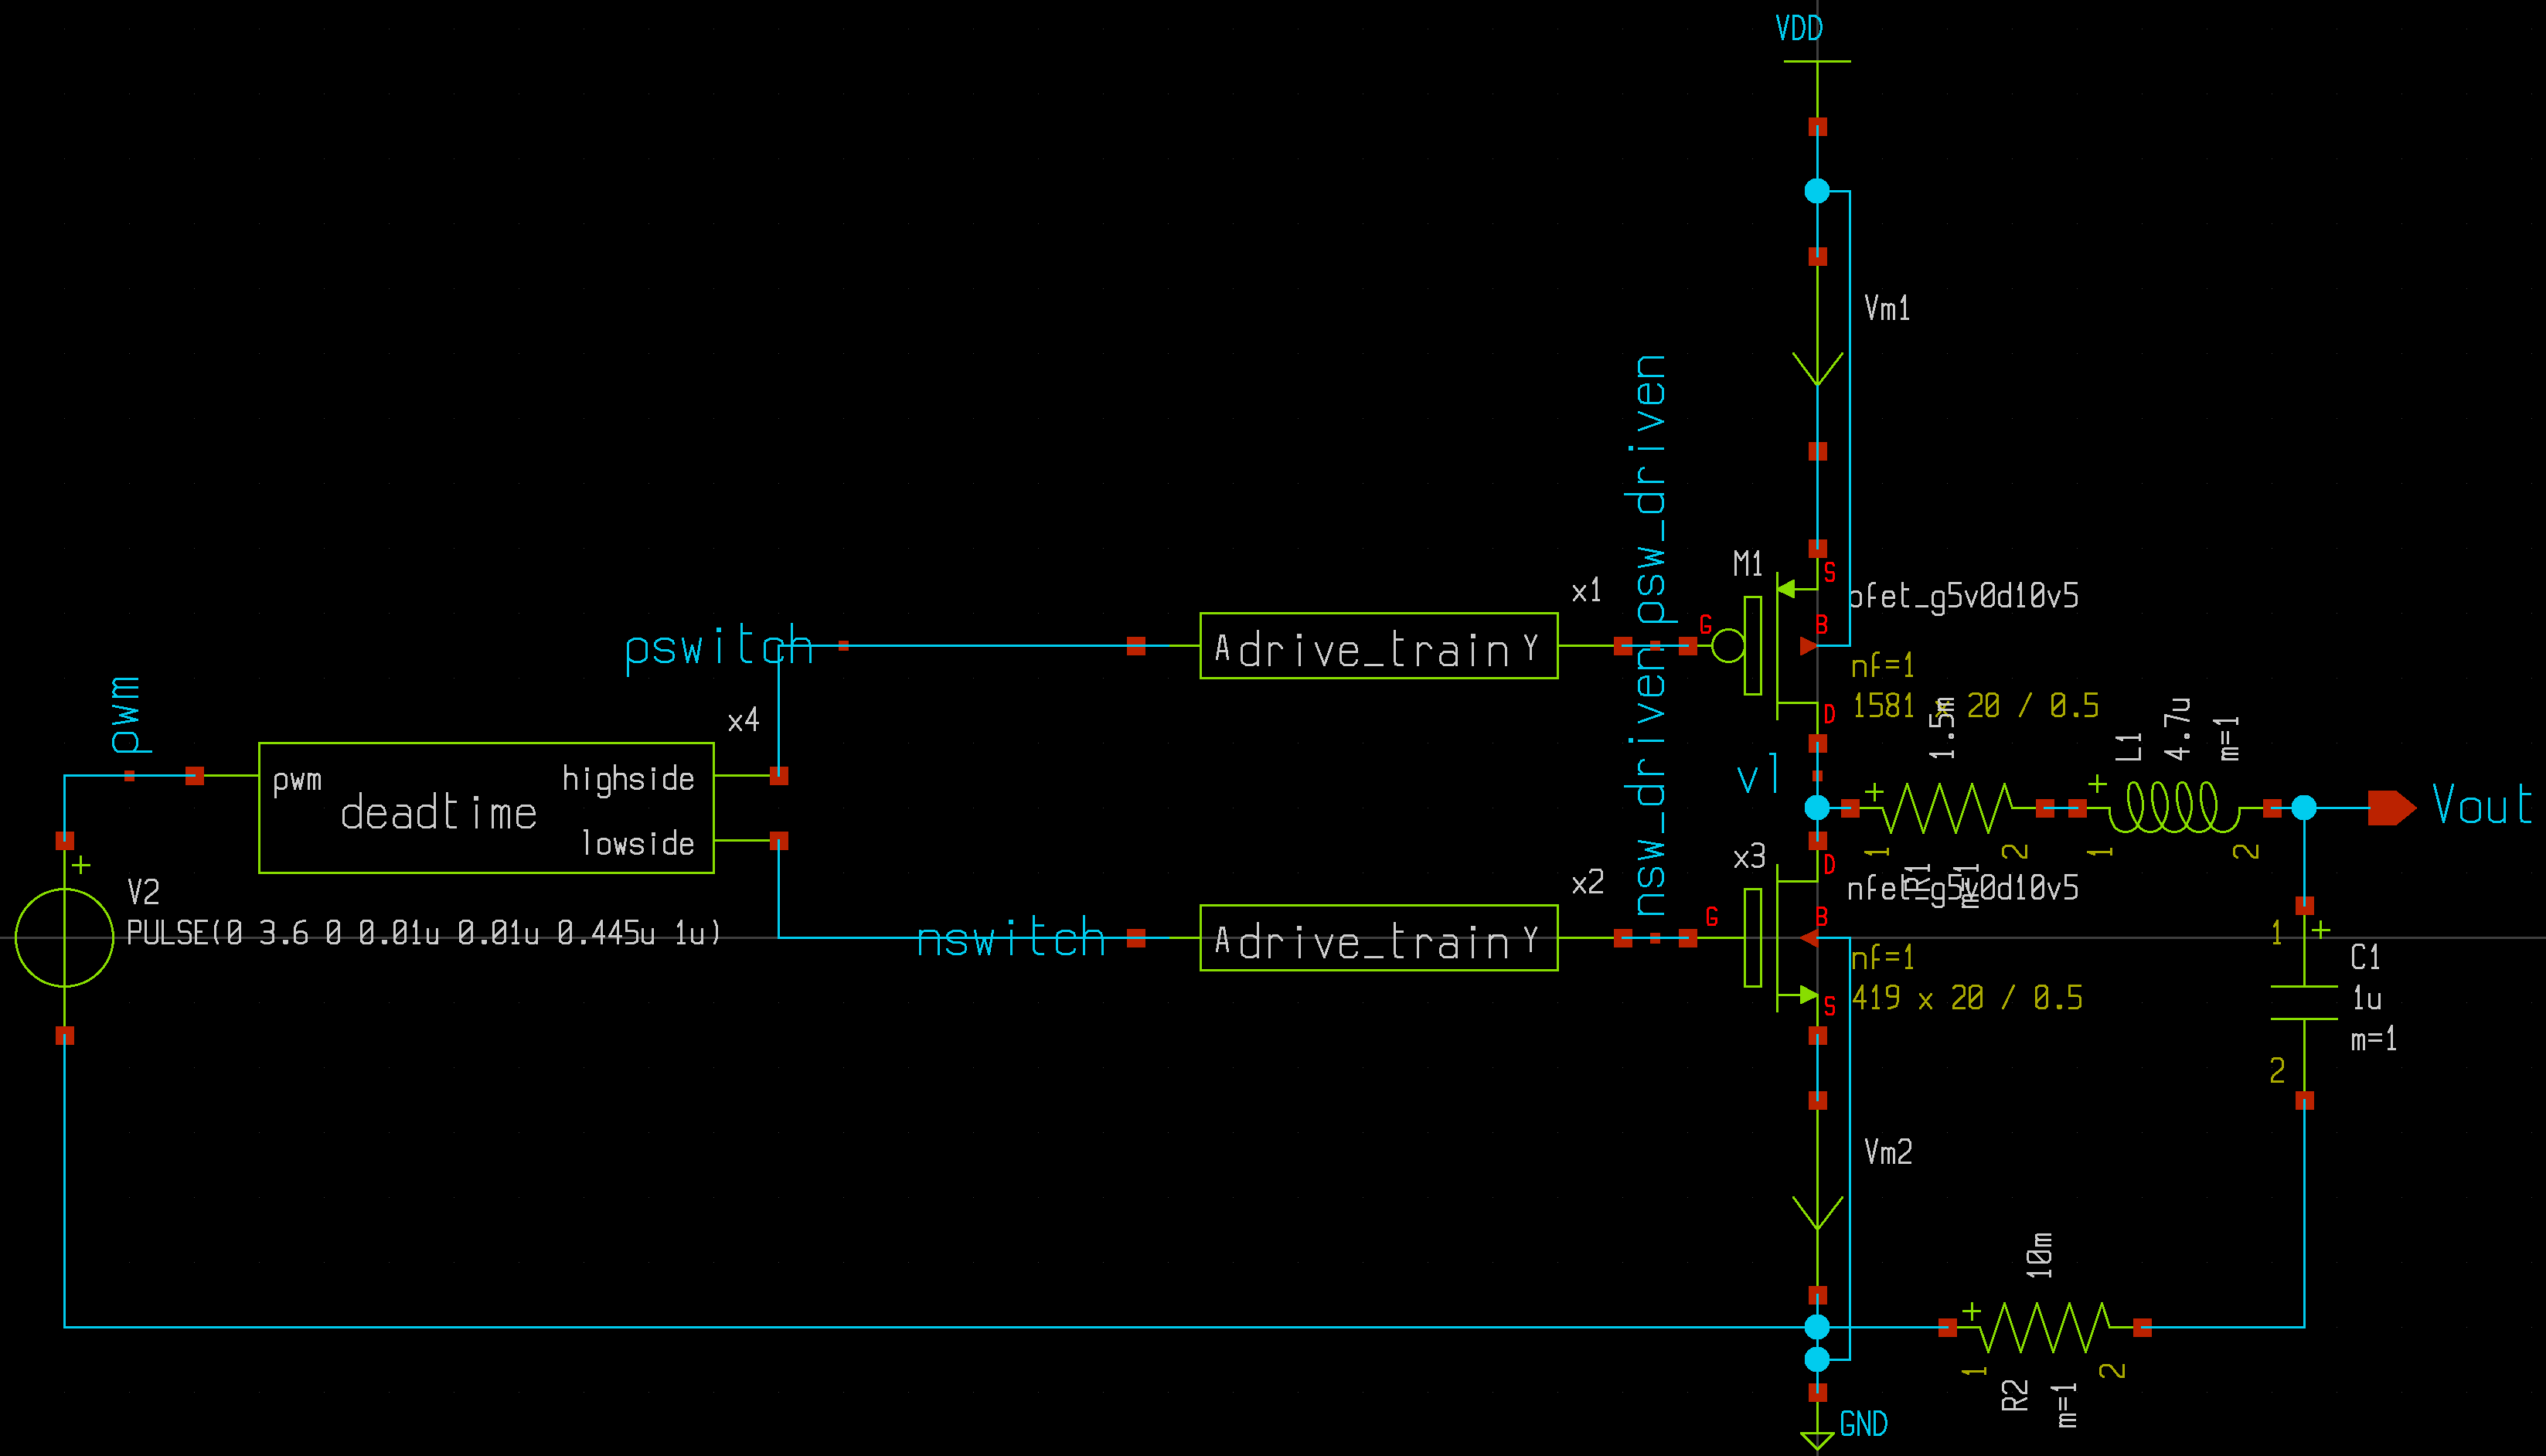
\includegraphics[scale=0.08]{buck.png}
\end{frame}

\begin{frame}
  \frametitle{Drive Train}
  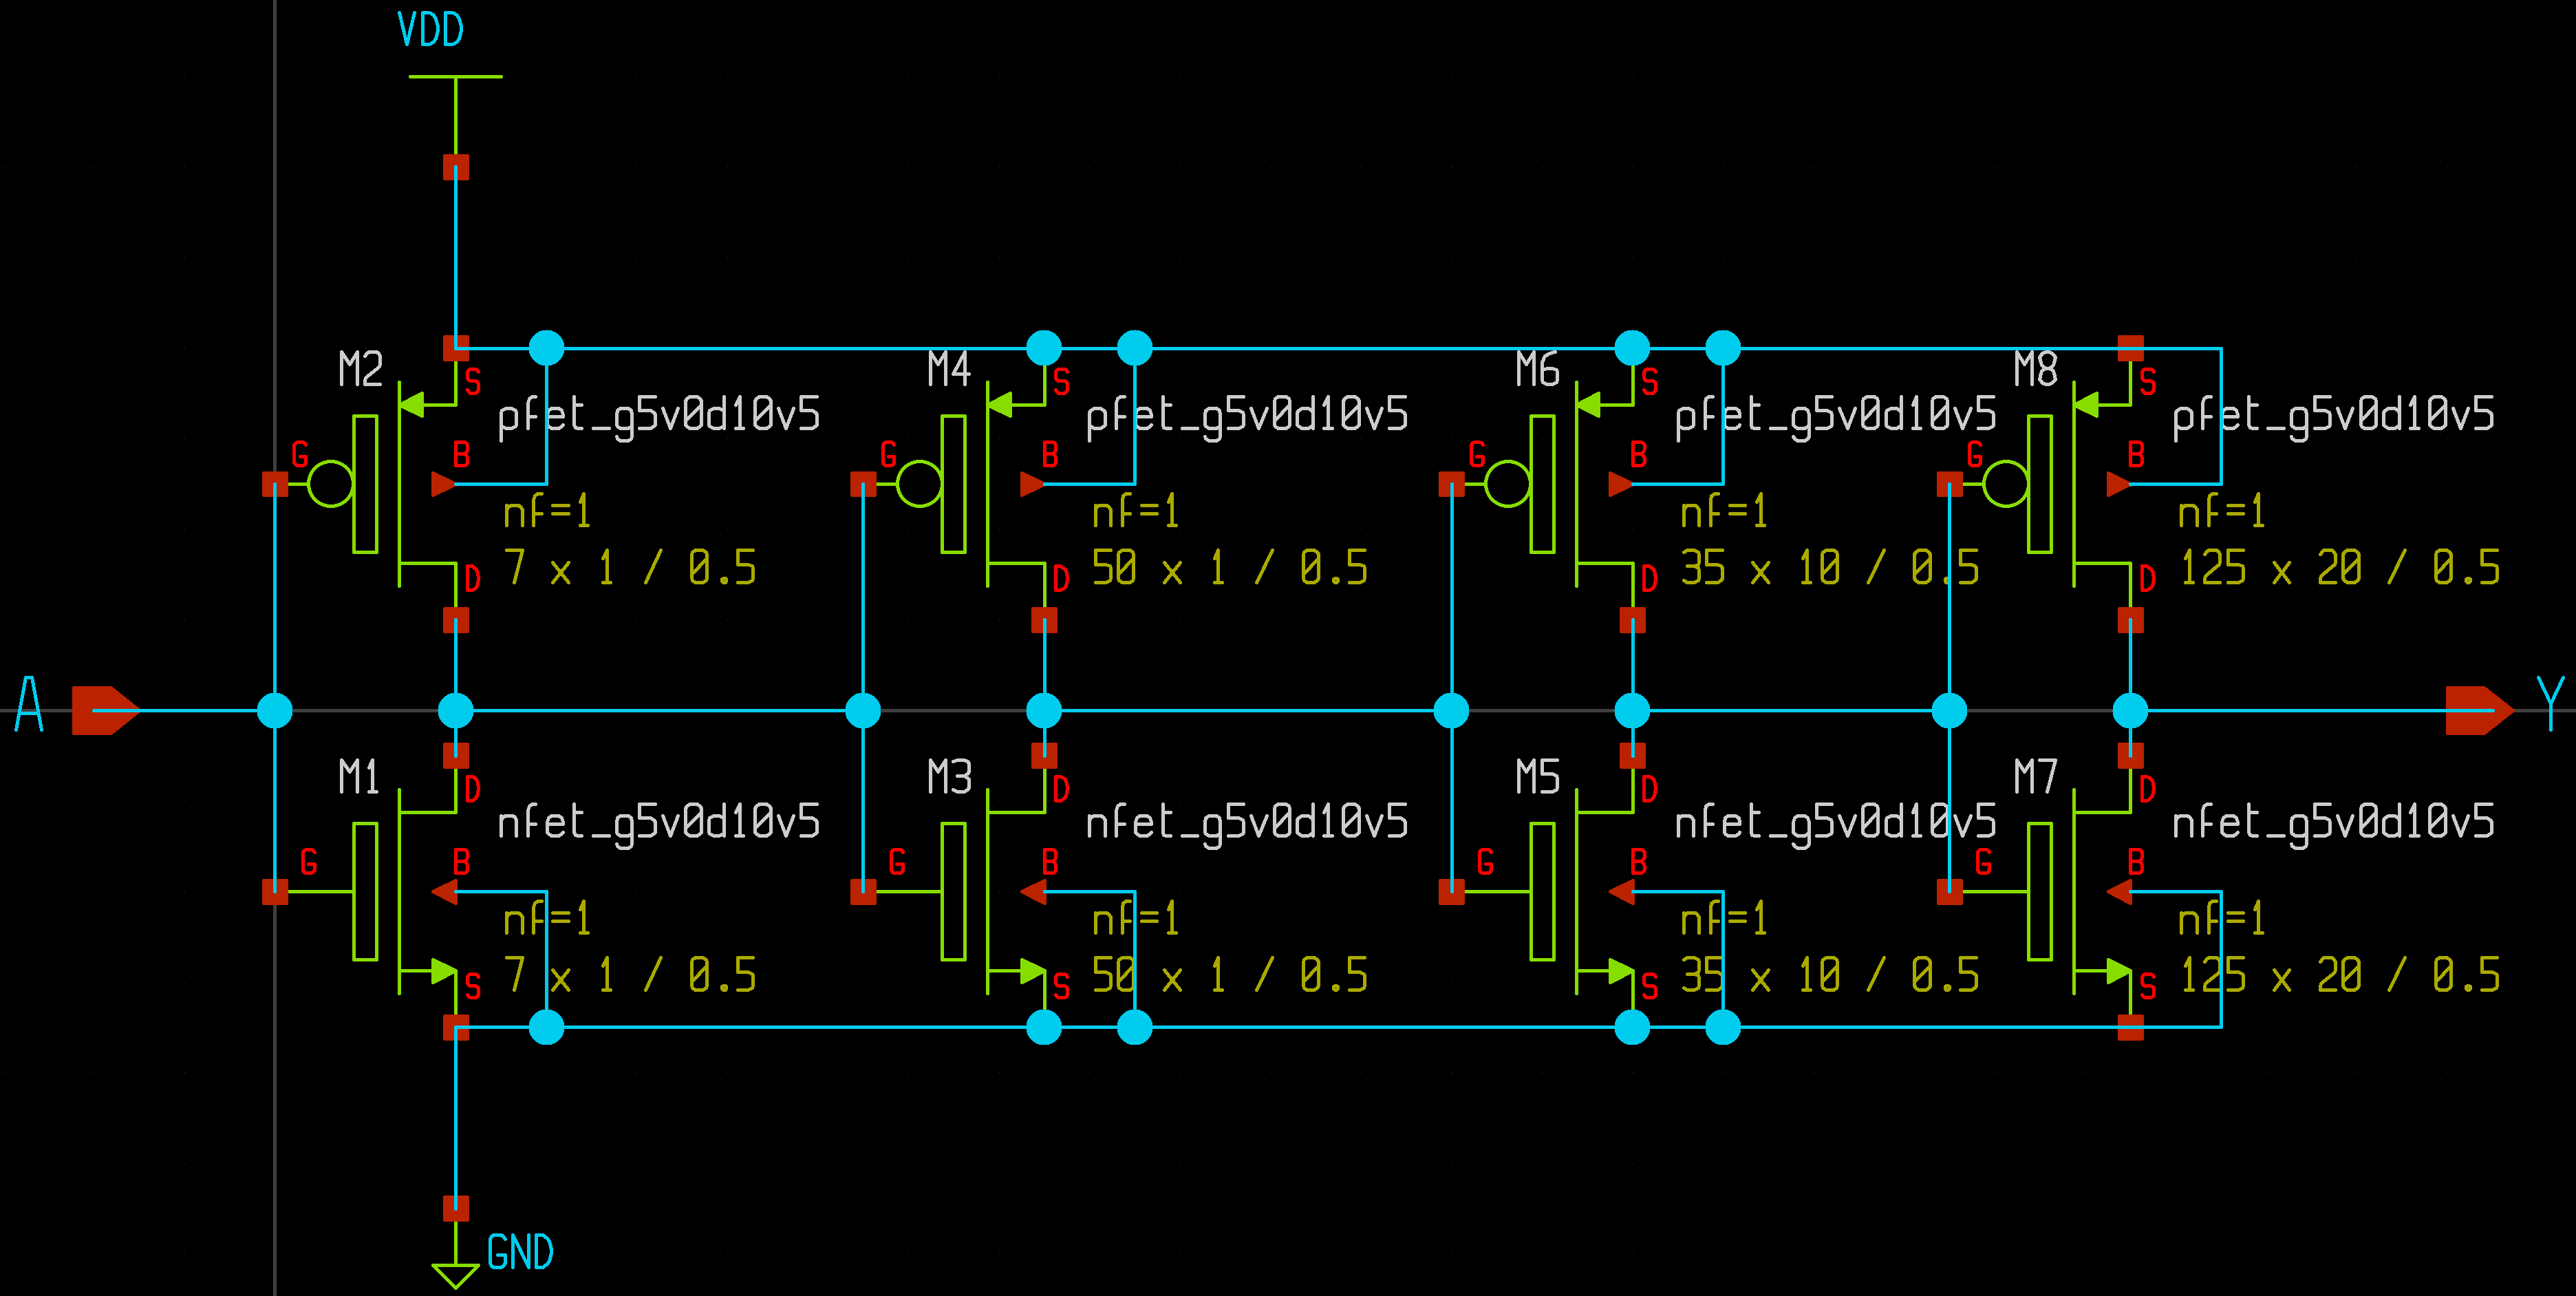
\includegraphics[scale=0.08]{drive-train.png}
\end{frame}

\begin{frame}
  \frametitle{Deadtime}
  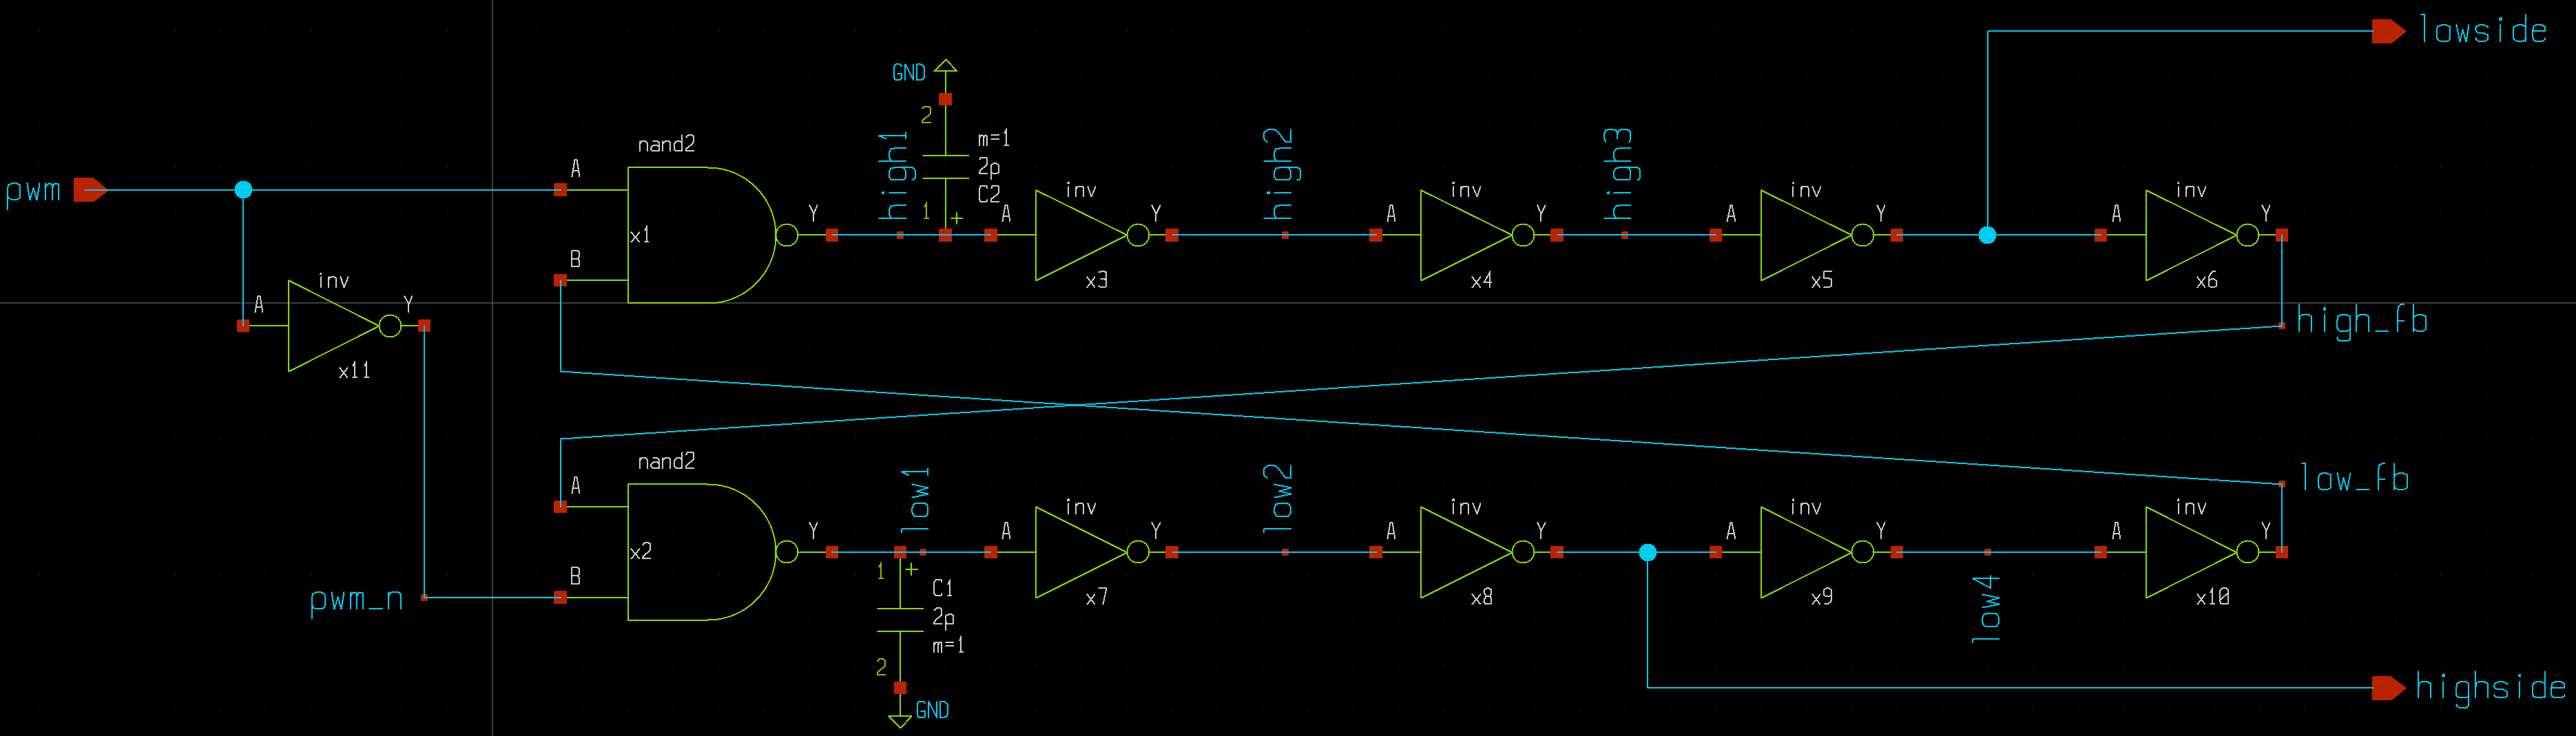
\includegraphics[scale=0.085]{deadtime.png}
\end{frame}

\begin{frame}
  \frametitle{Deadtime Inverter}
  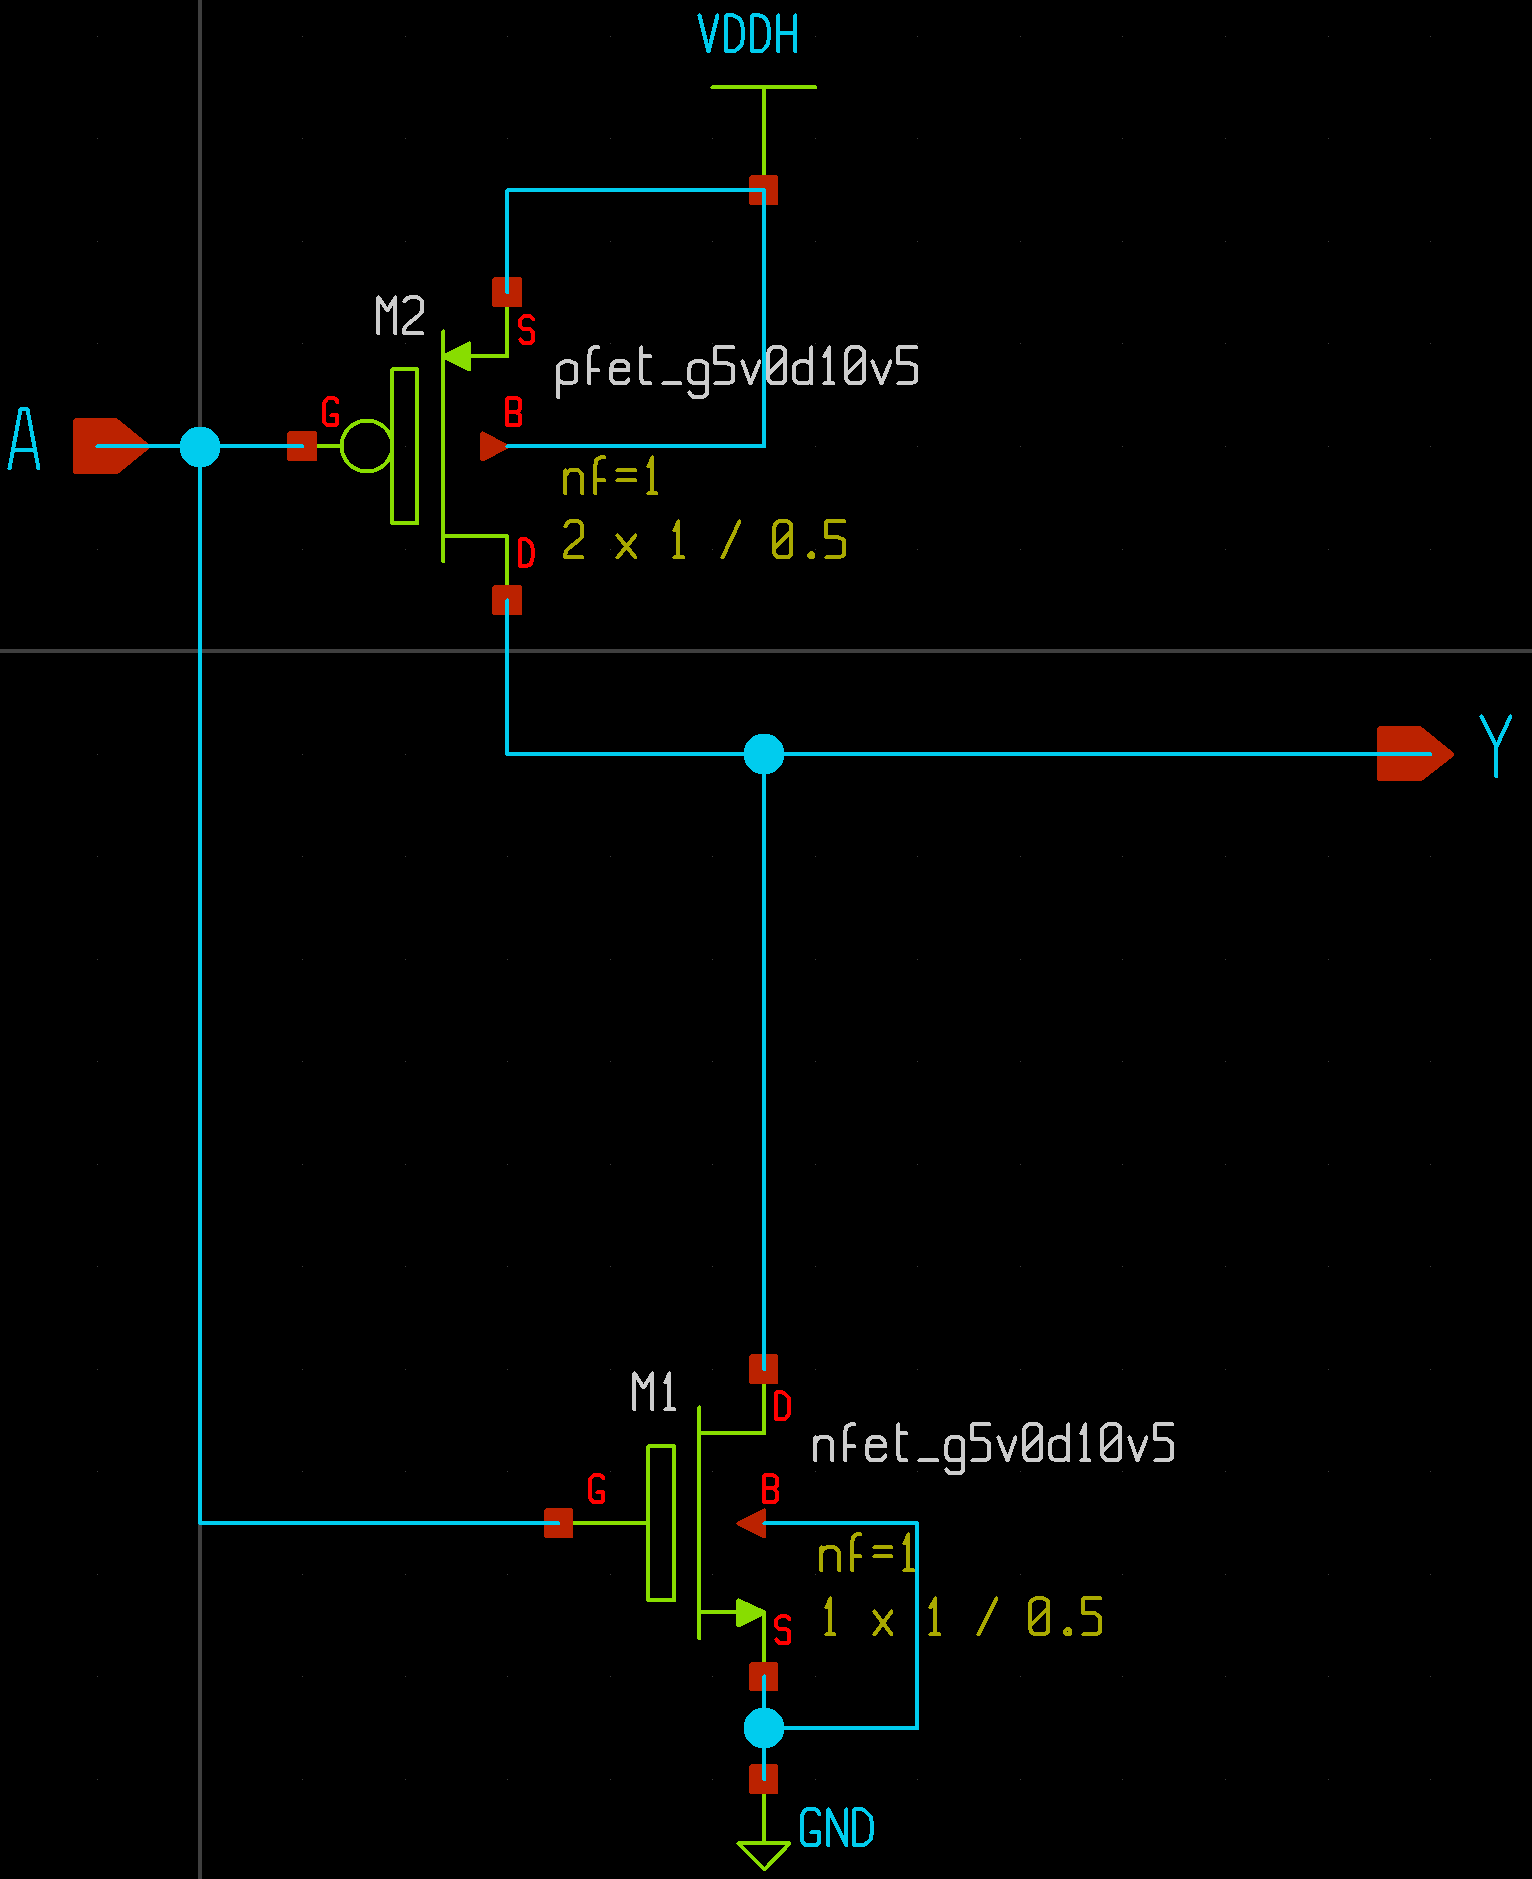
\includegraphics[scale=0.09]{inverter.png}
\end{frame}
\begin{frame}
  \frametitle{Deadtime Nand}
  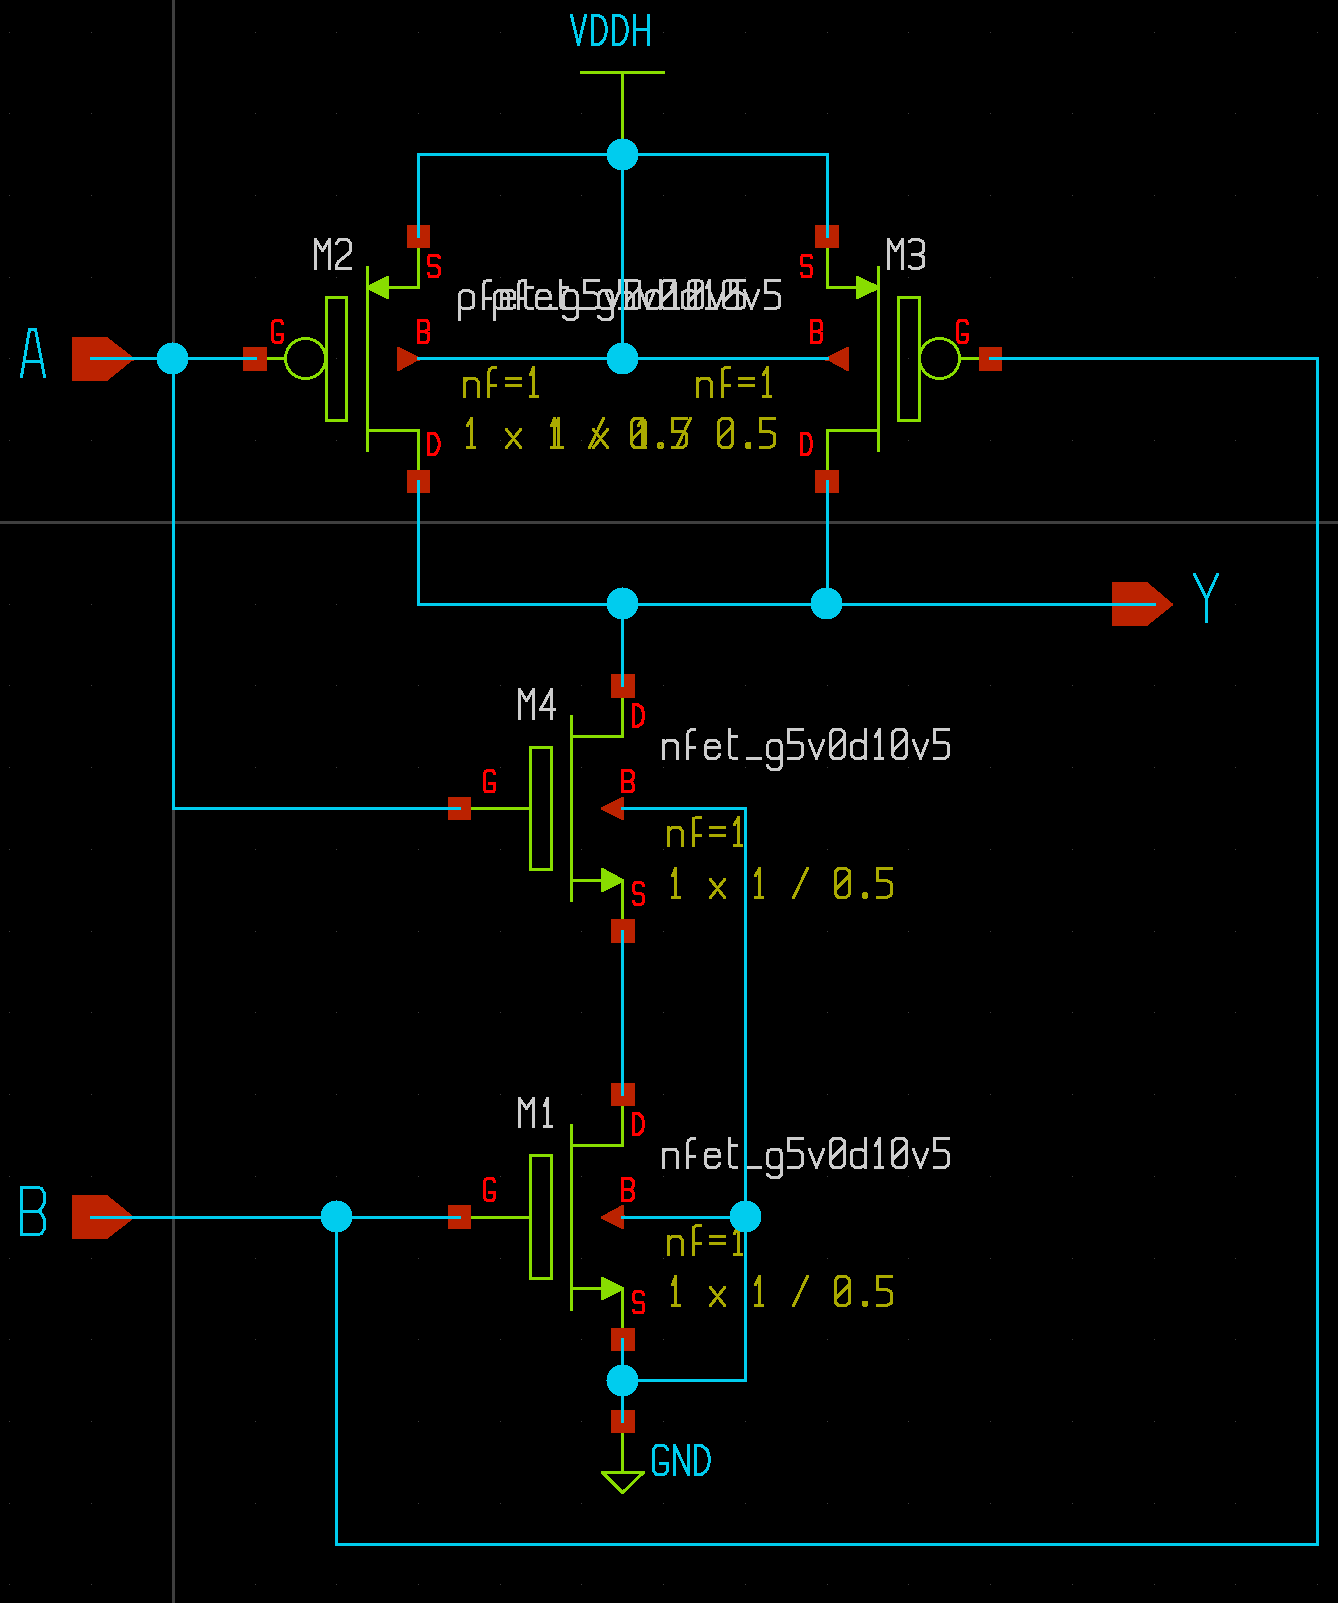
\includegraphics[scale=0.09]{nand.png}
\end{frame}

\begin{frame}
  \frametitle{Test Bench}
  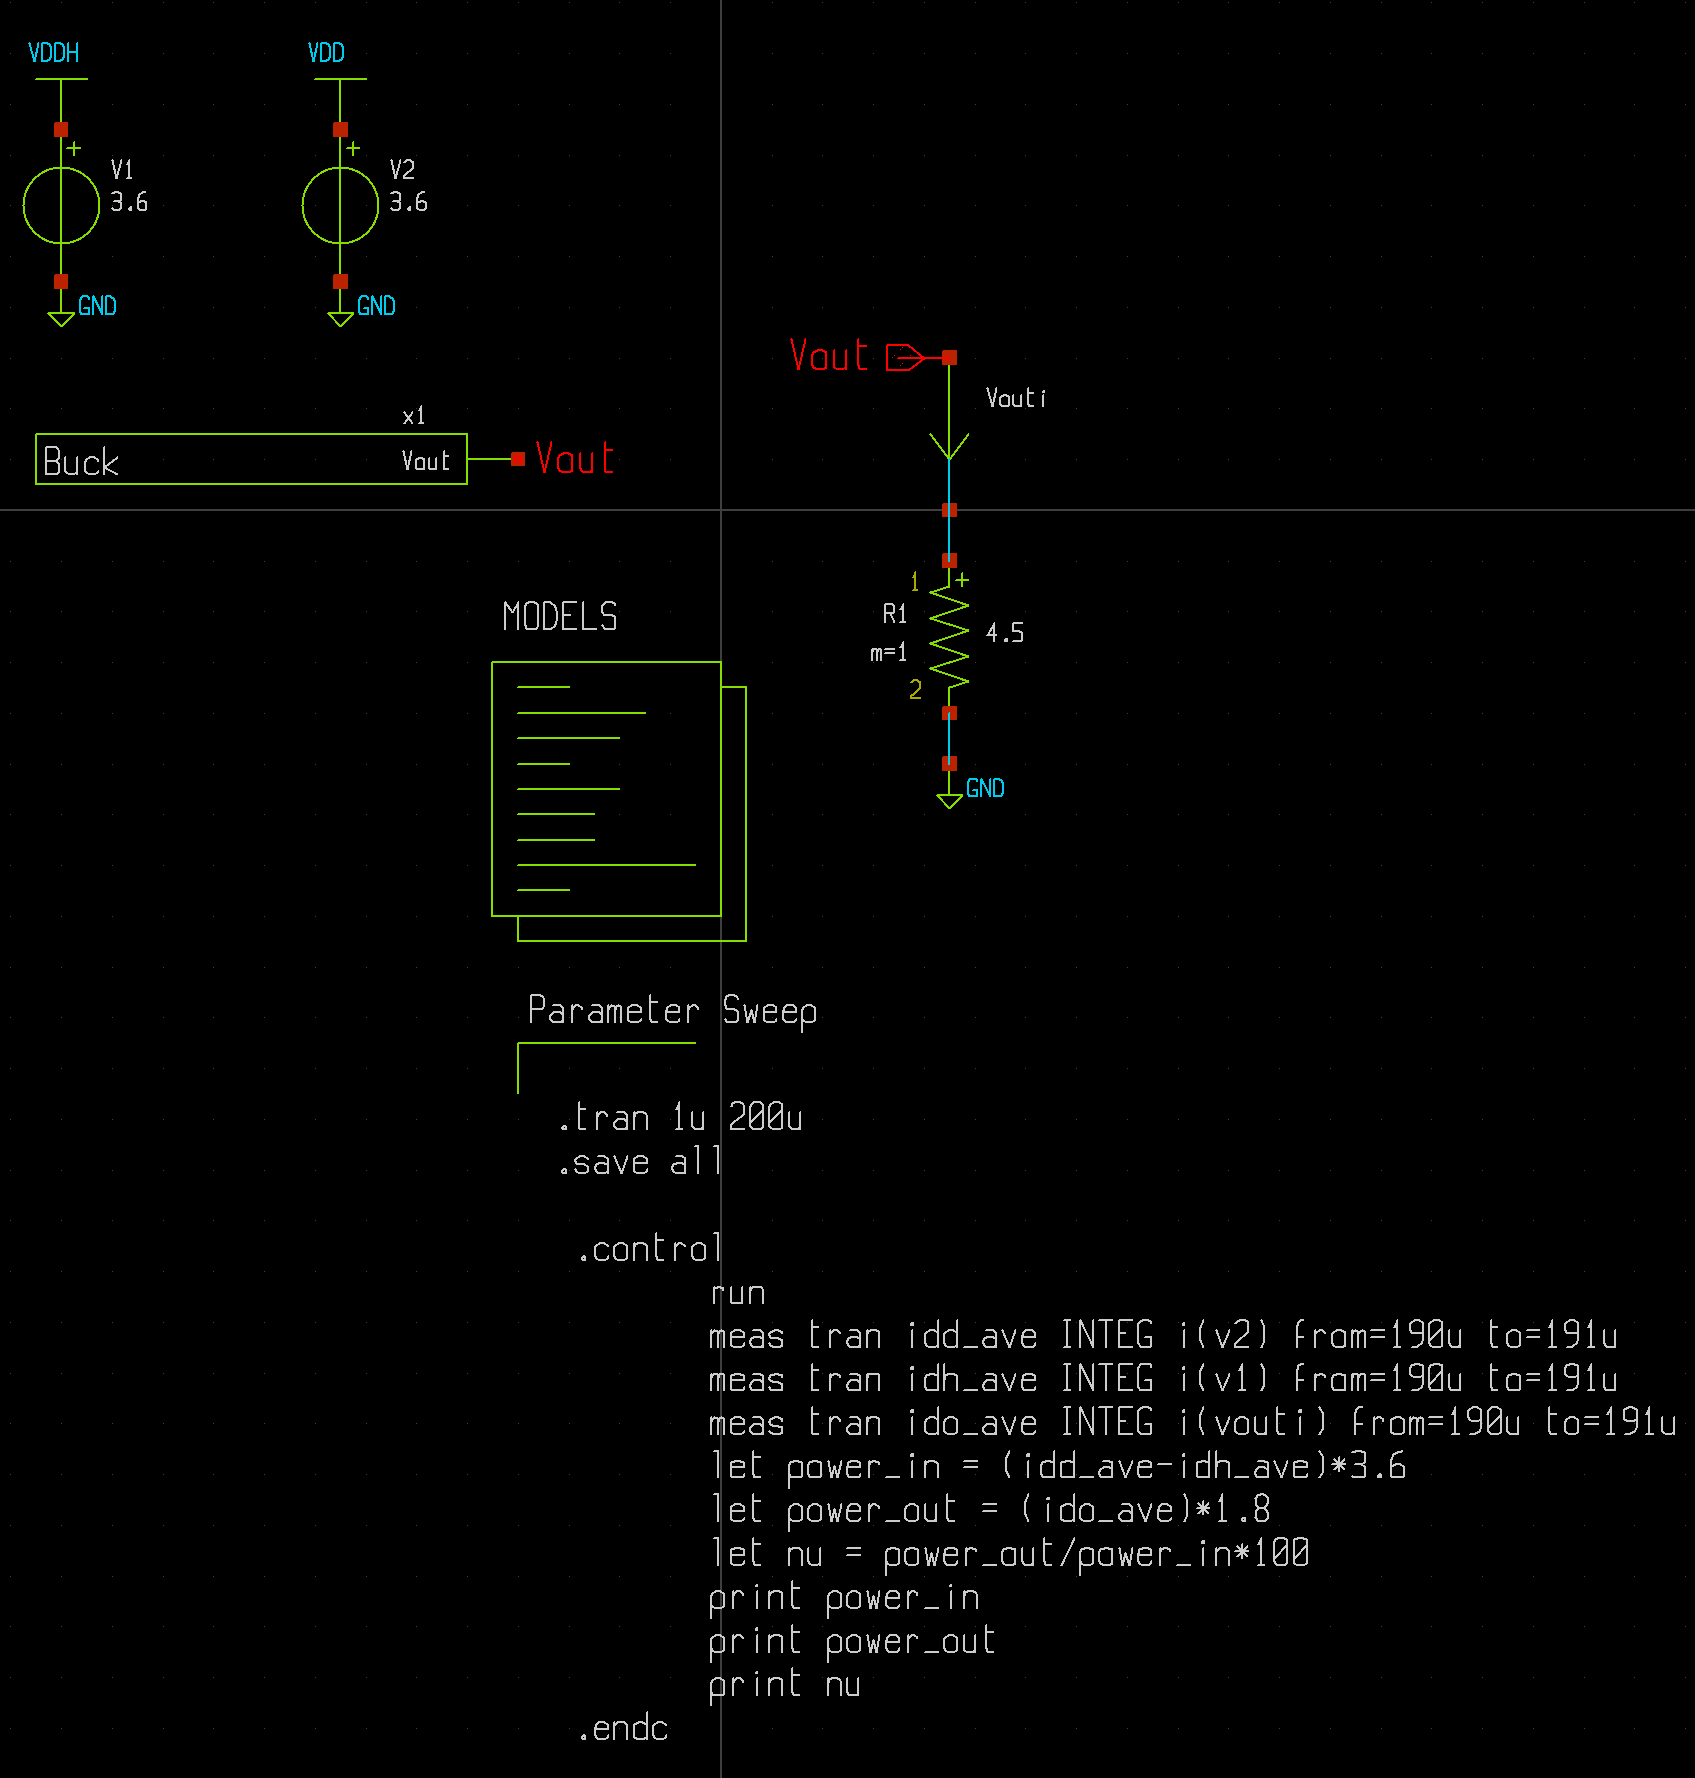
\includegraphics[scale=0.10]{testbench.png}
\end{frame}

\begin{frame}
  \frametitle{Efficiency}
\end{frame}

\begin{frame}
  \frametitle{Ripple}
\end{frame}



\end{document}
